\documentclass[aspectratio=169]{beamer}
\usetheme{Madrid}
\usecolortheme{beaver}
\usepackage[utf8]{inputenc}
\usepackage[T1]{fontenc}
\usepackage{tikz}
\usepackage{amssymb}
\usepackage{graphicx}
\setbeamertemplate{navigation symbols}{}
\setbeamercolor{title}{fg=white,bg=cyan!60!black}
\setbeamercolor{frametitle}{fg=white,bg=cyan!50!black}
\setbeamercolor{block title}{bg=cyan!15,fg=black}
\setbeamercolor{block body}{bg=cyan!5,fg=black}

\title{Story Studio 5 — Choose a Path}
\subtitle{if/else — a story that branches on the reader's choice}
\author{ByteForge --- Grade 7 --- Game Maker}
\date{}

\begin{document}

\begin{frame}
    \titlepage
\end{frame}

\begin{frame}{Today's Plan}
    \begin{itemize}
        \item Two Endings
        \item Three Paths
        \item Branch on the Click
        \item[$\bigstar$] BOSS --- Your Story, Your Ending
    \end{itemize}
\end{frame}

\begin{frame}{A variable is only useful if something CHECKS it}
    \Large
    A variable stores a choice; IF/ELSE is what actually MAKES that choice matter — without a branch, every choice would look the same.

    \begin{center}
    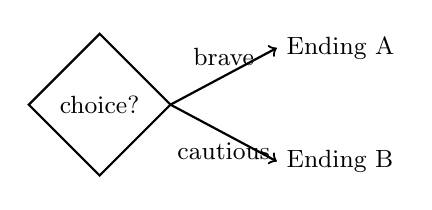
\begin{tikzpicture}[scale=0.9]

        \draw[thick] (1,1) -- (2,0) -- (1,-1) -- (0,0) -- cycle;
        \node at (1,0) {\small choice?};
        \draw[->, thick] (2,0) -- (3.5,0.8) node[midway, above] {\small brave};
        \draw[->, thick] (2,0) -- (3.5,-0.8) node[midway, below] {\small cautious};
        \node[right] at (3.5,0.8) {\small Ending A};
        \node[right] at (3.5,-0.8) {\small Ending B};
    \end{tikzpicture}
    \end{center}
\end{frame}


\begin{frame}{else if — a genuine third path}
    \Large
    Conditions are checked top to bottom, and the FIRST one that's true wins — order matters when ranges overlap.
\end{frame}


\begin{frame}{Branching on a value THAT JUST CHANGED}
    \Large
    Update the variable first, THEN check it — get the order backwards and the branch is always one click behind reality.
\end{frame}


\begin{frame}{BOSS — the whole semester, one real page}
    \Large
    Structure, style, behaviour, memory, decisions — a real interactive story needs genuinely all five.
\end{frame}

\begin{frame}{Real-World Example}
    \Large
    A "choose your own adventure" book, a Netflix interactive episode (Bandersnatch), or a game's dialogue choice — every branch a reader/player can take is an if/else somewhere in the code. Minecraft villagers branch too: trade with them enough and their dialogue/trades change — a real if/else on a "reputation" variable.
\end{frame}


\begin{frame}{Let Them Discover (1/2)}
    \Large
    Think of a choice-based story or game you know. Sketch its first three branches on paper as boxes and arrows (this is secretly a flowchart) before we build one in code.
\end{frame}


\begin{frame}{Let Them Discover (2/2)}
    \Large
    In Minecraft, trading with a villager enough times unlocks better trades. What do you think the game is checking each time — and what "branch" fires once you cross that threshold?
\end{frame}

\begin{frame}{Your Turn}
    \Large
    Open the student map, find \textbf{Story Studio 5 — Choose a Path}, and work through it
    hands-on --- everything you just saw, they now do themselves.
\end{frame}

\end{document}
